\chapter{Literature Review} 
\label{Chapter2}

The chapter provides an insight into the previous academic work completed in the field related to credit scoring and loan default prediction models. The chapter further describes machine statistical and machine learning used techniques to developed loan default prediction models. Finally the chapter describes the work related to using alternative features in credit scoring. 

%---------------------------------------------------------------------------------------
%	SECTION 1
%---------------------------------------------------------------------------------------

\section{Loan Default Prediction}

Throughout history consumer lending has grown more and more popular. The first recorded case of consumer lending dates back to the Babylonian period over 4000 years ago. Since then the creditworthiness of each credit applicant has been assessed. The birth of computers allowed for this process to be automated and allowed for credit models to be developed \parencite{CreditScoringIntroLewis}. \\

Credit scoring is defined as the scientific approach for assessing the creditworthiness of a potential borrower. This approach was first automated by D Durand in 1941. Durand developed a discriminant analysis model that classified potential borrowers into two distinct categories. Those unlikely to repay, and those likely to repay. This form of classification model is now refereed to as a loan default prediction model. These models form the heart of credit scoring systems. Durand's model not only speed up the process of loan default prediction but it also removed the need for subjective rules in the creditworthiness assessment process \parencite{CreditScoringIntroThomas}. \\

Durand's automated approach for assessing creditworthiness and was initially met with scepticism by the majority of the banking sector. It took until the late 1960s for credit scoring to be deemed the accepted method for assessing consumer creditworthiness. This was driven by two major developments. The introduction of credit cards and advances in the processing power of the era's computers. The introduction of credit cards led to a rapid rise in the number of consumers seeking credit, which meant that manually creditworthiness checks were no longer a valid option. The finical industry turned to automated models \parencite{CreditScoringIntroMarquez}. \\

Credit scoring models were rapidly developed throughout the 1970s and 1980s. Due to the precious nature of the credit scoring systems within lending companies, very little was released about the specific content used in the models and how the models were developed.   However, a number of models developed by academics were designed to represent the models and systems used within the industry during this era. Each type of model had its own statistical strengths and weaknesses \parencite{CreditScoringReadings}. \\

By the 1990s credit scoring models were regularly used to assess potential personal loans, business loans, and small loans. This decade also saw the introduction of credit score cards. In more recent times machine learning and artificial intelligence have been used in credit scoring. These models are far more complex than their predecessors and have not yet been fully accepted by regulatory bodies \parencite{CreditScoringTechniquesOverview}. \\

There are two main categories that credit scoring models can fit into. One category contains models driven by statistical learning techniques. The other contains models driven by machine learning techniques. Certain works completed in those categories will be discussed in the following sections. 

%---------------------------------------------------------------------------------------
%	SECTION 2
%---------------------------------------------------------------------------------------

\section{Statistical Credit Models}

A wide variety of statistical techniques have been used to develop effective and predictive credit scoring models. These techniques include weight of evidence measure, regression analysis, discriminant analysis, probit analysis, logistic regression, linear programming and decision trees. These techniques produce results than can be easily understood by regulators and communicated to other members of a business \parencite{CreditScoringTechniquesLitReview}. 

\subsection{Linear Discriminant Analysis}

Linear Discriminant Analysis (LDA) is a simple parametric statistical technique that is used to distinguish between two classes. In terms of credit scoring, LDA is used to classify potential borrowers into one of two classes, a class containing borrowers that are likely to repay or a class containing borrowers that are unlikely to repay. LDA is still one of the most broadly established techniques in credit scoring and loan default prediction. It was first used as a credit scoring approach by \textcite{DurandLDA}. \\

Durand developed an LDA model with the following linear discriminate function.

\vspace{15pt}

\begin{equation} \label{eq:LDA}
LDF = a_{0} + a_{1}x_{1} + a_{2}x_{2}+ ... +  a_{n}x_{n}
\end{equation}

\vspace{15pt}

Where $x_{1}$ ... $x_{n}$ represent the variables use to classify potential borrows and $a_{1}$ ... $a_{n}$ indicate the discrimination coefficients for the variables. The \ref{eq:LDA} returns a a single numeric value. A potential borrower is classified as likely to pay or not based upon the value being above our below a predefined cut-off value. \\

The variables used in Durand's model were an applicants age, their sex, their residential status, their occupation, the field of industry the applicant worked in, the number of years the applicant had worked at their current employer, and Boolean variables indicating whether or not the applicant had a bank account, real estate and life insurance. Each variable was bucketed into different categories and each category was a assigned a value. The minimum and maximum values of Durand's formula where 0 and 3.46 respectively. Applicants that had a score less than 1.25 were denied credit \parencite{DurandLDA}.  \\

LDA models have been scrutinised as they assume linear relationships
between dependent variables and independent variables. Furthermore, LDA models require the assumption to be made that all input variables must follow a Normal distribution \parencite{CreditScoringTechniquesOverview}. \newpage

\subsection{Logistic Regression}

Logistic regression was developed by David \textcite{LogReg}. Like LDA, logistic regression is an adaptation of linear regression. However, logistic regression does not require the same assumptions to be made about the variables used. \\

The technique is used to describe the relationship between one dependent binary variable and one or more nominal, ordinal, interval or ratio-level independent variables. Logistic regression models always produce dichotomous results (values are either 0 or 1) and have been widely used to solve binary classification problems. \\

\textcite{LogRegWiginton} published one of the first works relating to using a binary classification logistic regression model in credit scoring. The model he developed was based on the following cumulative logistic probability function.

\vspace{15pt}

\begin{equation} \label{eq:LR}
ln(\frac{p_{i}}{1-p_{i}}) = \beta_{0} + \beta_{1}x_{1} + \beta_{2}x_{2}+ ... +  \beta_{n}x_{n}
\end{equation}

\vspace{15pt}

Where $p_{i}$ is the probability of customer defaulting on a potential credit, $\beta_{i}$ are the coefficients of the input variables and $x{i}$ are the input variables. \\

Wiginton developed an optimal cut-off probability that was used to assign potential borrowers to either a "bad creditors" class or a "good creditors" class. Those assigned to the "bad" class were not granted credit.  \\

A visual representation of Wiginton's model can be seen in figure \ref{fig:LR}. The summation symbol represents equation \ref{eq:LR}, while the sigmoid function represents the binary cut-off.  

\vspace{15pt}

\begin{figure}[!htb]
\centering
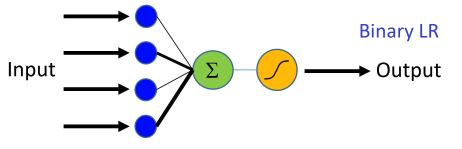
\includegraphics[width = \textwidth]{images/logistic_reg.png}
\caption{Wiginton's Logistic Regression Model}
\parencite{LogRegFig}
\label{fig:LR}
\end{figure}

\vspace{15pt}

Wiginton deemed that a logistic regression model gave superior classification results when compared to a LDA model. His model was able to achieve a classification accuracy of over 58\%. However, \textcite{LogRegHand} compared using logistic regression approach to simple linear regression and found that both approaches had very similar classification accuracies. 

\subsection{Classification Tress}

Classification and Regression Trees (CART) are another statistical technique that have been commonly used for credit scoring. Like LDA and logistic regression, they have been used to classify potential borrowers into either a "likely to repay a financial obligation" or "unlikely to repay a financial obligation" class. They are non-parametric models used to predict a dependent variable as a function of continuous independent variables. Decision trees are dichotomous models that are developed by splitting the records at each node based on a function of a single input. They consider all possible splits and identify the best sub-tree based on its overall error rate \parencite{DecTreesZekic}. \\

The CART algorithm was developed by \textcite{DecTreesBrieman}. They found that CART models are invariant under transformations in the predictor space and that Multi-factor response is easily dealt with. Furthermore, they found that modelling results could be easily to explained to non-statisticians due to their CART's inherent visual properties. Figure \ref{fig:CART} displays the algorithm developed by \textcite{DecTreesBrieman}. 

\vspace{15pt}

\begin{figure}[!htb]
\centering
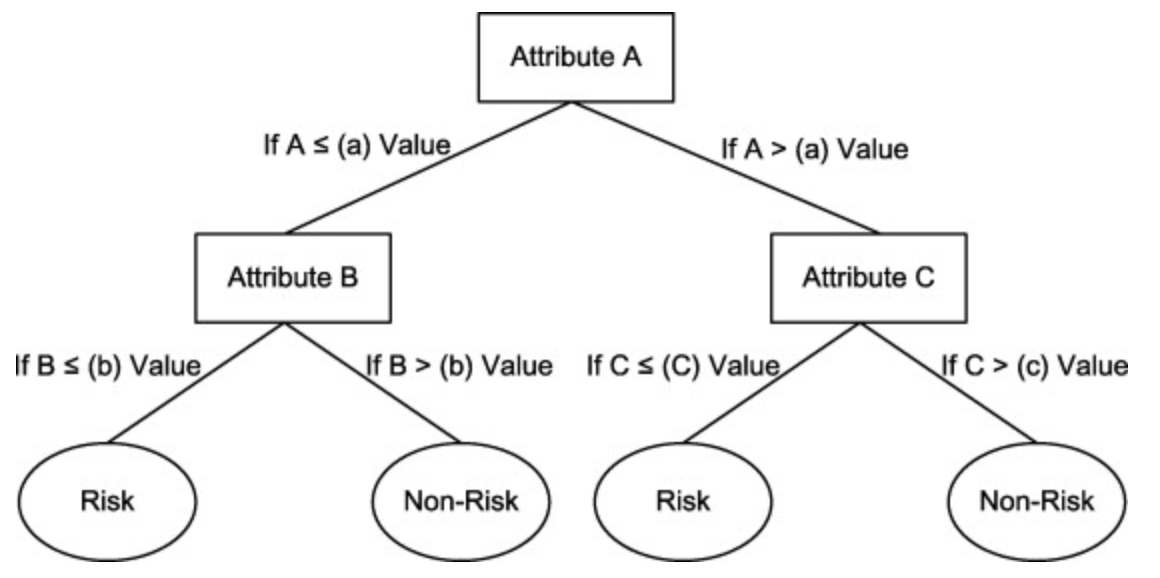
\includegraphics[width = \textwidth]{images/CART.png}
\caption{CART Model}
\parencite{DecTreesBrieman}
\label{fig:CART}
\end{figure}

\vspace{15pt}

In figure \ref{fig:CART} the subset branches created by each split are ref referred to as nodes. The subsets which are not split are named terminal nodes. Terminal nodes get assigned to one of the predefined classes. In figure \ref{fig:CART} there are 3 classes. A predicted classes for an input vector is found by passing through each binary node in the tree until a terminal node is reached. \\

\textcite{DecTreesZekic} compared the performance of a CART, a neural network (NN) and logistic regression model in scoring a sample small business loans provided by a Croatian bank. They used pruning to avoid over-fitting. A technique that involves growing a tree and then removing branches and terminal nodes that do not contain a predefined number of data points. They used Gini index as the evaluation function used for splitting. \newpage


Gini index is calculated as shown in equation \ref{eq:GINI}. 

\vspace{15pt}

\begin{equation} \label{eq:GINI}
\sum_{j!=k}p_{ij}p_{ik} = 1 - \sum_{k}p_{ik}^{2}
\end{equation}
\vspace{15pt}

Where p represents the independent variables. \\


The results of \textcite{DecTreesZekic} research can be seen in table \ref{table:CART}. \\


\begin{table}[H]
\begin{center}
\begin{tabular}{|c|c|c|c|} 
\hline
\multicolumn{1}{|c}{Model}  &\multicolumn{1}{|c|}{Total Accuracy (\%)}  &\multicolumn{1}{|c|}{Bad Accuracy (\%)} & \multicolumn{1}{c|}{Good Accuracy (\%)}\\
\hline
Probabilistic NN & 83.30 &  80.00 & 85.19 \\
\hline
Logistic regression & 57.14 &  66.67 & 51.85 \\
\hline
CART & 66.67 &  66.67 & 66.67 \\
\hline
\end{tabular}
\end{center}
\caption{Results of Research Conducted by \textcite{DecTreesZekic} }
\label{table:CART}
\end{table}

\vspace{15pt}

The models displayed in Table \ref{table:CART} were trained on the same training data and the same 20 variables. It can be seen from Table \ref{table:CART} that the CART model produced by \textcite{DecTreesZekic} outperformed their logistic regression model in terms of total accuracy and in terms of predicting loans that were repaid (Good Accuracy). However, the CART model was outperformed in predicting both loan that were not repaid (Bad Accuracy), loans there were not repaid and over all accuracy by their probabilistic NN model.  

%---------------------------------------------------------------------------------------
%	SECTION 3
%---------------------------------------------------------------------------------------
\section{Machine Learning Models}

After the rapid expansion of consumer credit numerous statistical methods were successfully used for credit risk assessment. However, these models often had difficulty in modelling complex financial scenarios due to their use of fixed functions and statistical assumptions \parencite{AICredDefSwap}. Studies have shown that machine learning techniques such as Support Vector Machines (SVM's), Random Forests , and Neural Networks are superior to that of statistical techniques in terms of predicting whether consumers are likely to repay a loan when the training sample is large \parencite{SVMCrook}. 


\subsection{Support Vector Machines}

SVM models define a hyper-plane that best separates two data classes so that the margin width between the hyper-plane and
the data points is maximised. The hyper-plane can be linear or non-linear. The wider the  margin width, the less complex the model is and the more likely it is to generalise well. \\


The hyper-plane can often be difficult to define if the classes are not well separated. Figure \ref{fig:SVM} displays such a case. \newpage

\vspace{15pt}

\begin{figure}[!htb]
\centering
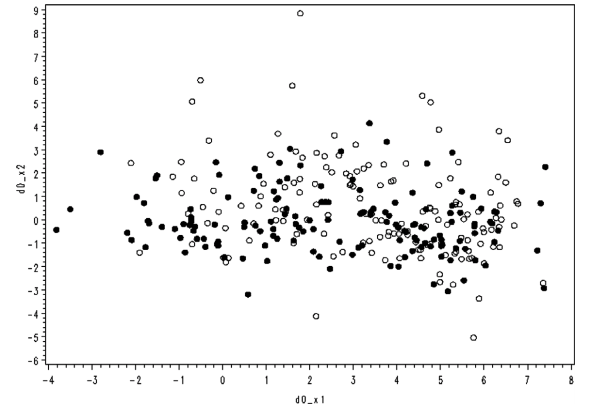
\includegraphics[width = 0.9\textwidth]{images/SVM.png}
\caption{Poorly Separated Credit Data}
\parencite{SVMCrook}
\label{fig:SVM}
\end{figure}

\vspace{15pt}


\textcite{SVMCrook} developed a SVM model that predicted whether credit card users would default on their repayments. A consumer was deemed to have defaulted if they fell more than 3 months behind on their repayments within the first 12 months of their account opening. They used a training sample of 25,000 consumers. The model developed used a a non-linear kernel and its parameters were tuned using a grid search in order to maximise the model's area under the Receiver operating characteristic curve (AUC), which is a single summary statistic used to measure a binary classification model's specificity (true negative rate) and sensitivity (true positive rate). \\

On top using the SVM model to classify loans, \textcite{SVMCrook} used the magnitude of the weight of each feature as a feature selection criterion. They only included features with a weight of more than 0.1 in their final model. They compared their SVM model to a logistic regression and k-nearest neighbours (KNN) model. They compared each model's AUC, sensitivity and specificity. Figure \ref{fig:SVMLR} compares the performance of SVM model to the performance of the logistic regression model, while figure \ref{fig:SVMKNN} compares the performance of SVM model to the performance of the KNN model. In both figures the solid line is the SVM model's performance and the broken line is the other model. \\

We can see from figures \ref{fig:SVMLR} and \ref{fig:SVMKNN} that the SVM model outperformed the other model. Furthermore, the SVM model had a better training and test AUC, specificity , and sensitivity than the other two models. 

\vspace{15pt}

\begin{figure}[!htb]
\centering
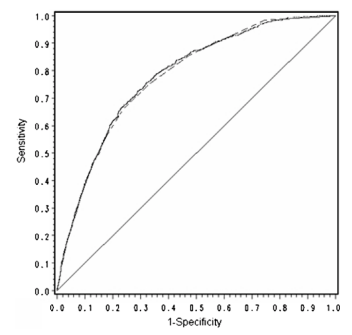
\includegraphics[width=0.7\textwidth]{images/SVMLR.png}
\caption{SVM Model vs Logistic Regression Model}
\label{fig:SVMLR}
\end{figure}

\begin{figure}[!htb]
\centering
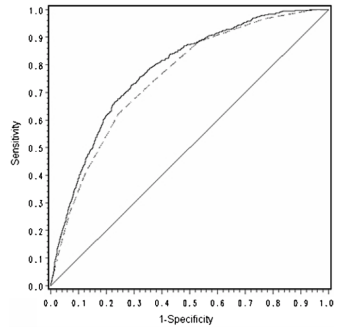
\includegraphics[width=0.7\textwidth]{images/SVMKNN.png}
\caption{SVM Model vs KNN Model}
\label{fig:SVMKNN}
\end{figure}

\vspace{15pt}

\subsection{Neural Networks}

The research conducted by \textcite{DecTreesZekic} displayed that neural networks improved on classification accuracy of more traditional statistical techniques such as decision trees and logistic regression when classifying whether or not consumers would repay a financial obligation. The research conducted by \textcite{NNWest} compared the performance, of five different neural network models, when they are applied to credit scoring.  The models developed varied in architecture, loss functions, and learning rates.  \\

West developed models with the following features: a multi-layer perceptron (MLP) model, a model that used the mixture-of-experts (MOE) approach, a model that used a radial basis function (RBF), learning vector quantization (LQV) model, and fuzzy adaptive resonance (FAR) model. The architectures of each model were made similar. The input and of and output layers of each model were identical. However, the hidden layer of each model varied. West determined the optimal number of nodes in the hidden layer of the MLP and MOE models using a cascade learning approach. The hidden layer layer of the LQV model was determined by setting the number of neurons in the layer equal to 10\% of the size of the training data. The hidden layers of the RBF and RAF models were determined experimentally.  \\

West used a sample of 1000 loans, provided by a German credit provider, to train and test the models he developed. The sample consisted of 700 loans that were repaid and 300 that were not. He used the same features to train each model and used 10-fold cross validation to test the accuracy of each model. 10-fold cross validation involves partitioning the training sample of a model into 10 partitions. One partition serves as an independent holdout test set for the credit model being trained while the remaining nine partitions are used to train the model. This technique minimises the effects of data dependencies and improves the reliability of the estimates. \\

Table \ref{table:NN} displays the results of West's research. Like Table \ref{table:CART}, Table \ref{table:NN} displays each model's accuracy in terms of predicting loans that were repaid, loans that were not repaid ,and overall prediction accuracy. The accuracies show are the average of the best three results from the 10-fold cross validation conducted for each model. 

\vspace{15pt}

\begin{table}[H]
\begin{center}
\begin{tabular}{|c|c|c|c|} 
\hline
\multicolumn{1}{|c}{Model}  &\multicolumn{1}{|c|}{Total Accuracy (\%)}  &\multicolumn{1}{|c|}{Bad Accuracy (\%)} & \multicolumn{1}{c|}{Good Accuracy (\%)}\\
\hline
MLP & 87.09 &  46.92 & 75.04 \\
\hline
MOE & 86.99 &  55.43 & 77.57 \\
\hline
RBF & 85.76 &  51.79 & 75.63 \\
\hline
LQV & 79.15 &  55.20 & 72.20 \\
\hline
FAR & 70.92 &  58.14 & 62.29 \\
\hline
\end{tabular}
\end{center}
\caption{Results of Research Conducted by \textcite{NNWest}}
\label{table:NN}
\end{table}

\vspace{15pt}

Table \ref{table:NN} displays that the MOE model is the best overall performing model. \textcite{NNWest} used a chi-square test to assess whether or not there were significant differences between the models he developed in terms of predicting loan default. The chi-square test indicated that MOE, RBF, and MLP are superior models for predicting loan repayment when compared to RAF and LQV models. \\

Table \ref{table:NN} does not show that West developed logistic regression and CART models as reference models. These models outperformed all neural network models, but were deemed significantly similar to the MOE, RBF, and MLP models. The reason for the strong performance of the statistical approaches was deemed to be due to the size of training set used to develop the models.  \\

\textcite{NNShen} used the same dataset as \textcite{NNWest} to train and test a back propagated neural network. Their model used a particle swarm optimisation (PSO) algorithm to search for the optimal weights and deviations in the BP neural network. \\

Further more, they used synthetic minority over-sampling technique (SMOTE) to balance the training dataset before the training the model. This was done as the majority of  credit history datasets are imbalanced towards the class containing customers that repaid their financial obligations. SMOTE involves generating synthetic examples of data points that belong to the minority class in a training dataset. \textcite{NNShen} generated synthetic examples by identifying the k nearest neighbours of a randomly selected minority data point. A variable difference vector between the minority instance under consideration and its corresponding nearest neighbours was then calculated and multiplied using a by a random value between 0 and 1. The feature vector was then added to the original minority data point. This process was completed until the ratio of credit defaulters and credit re-payers matched. Figure \ref{fig:smote} visually displays the steps carried out in the class balancing process. 

\vspace{15pt}

\begin{figure}[!htb]
\centering
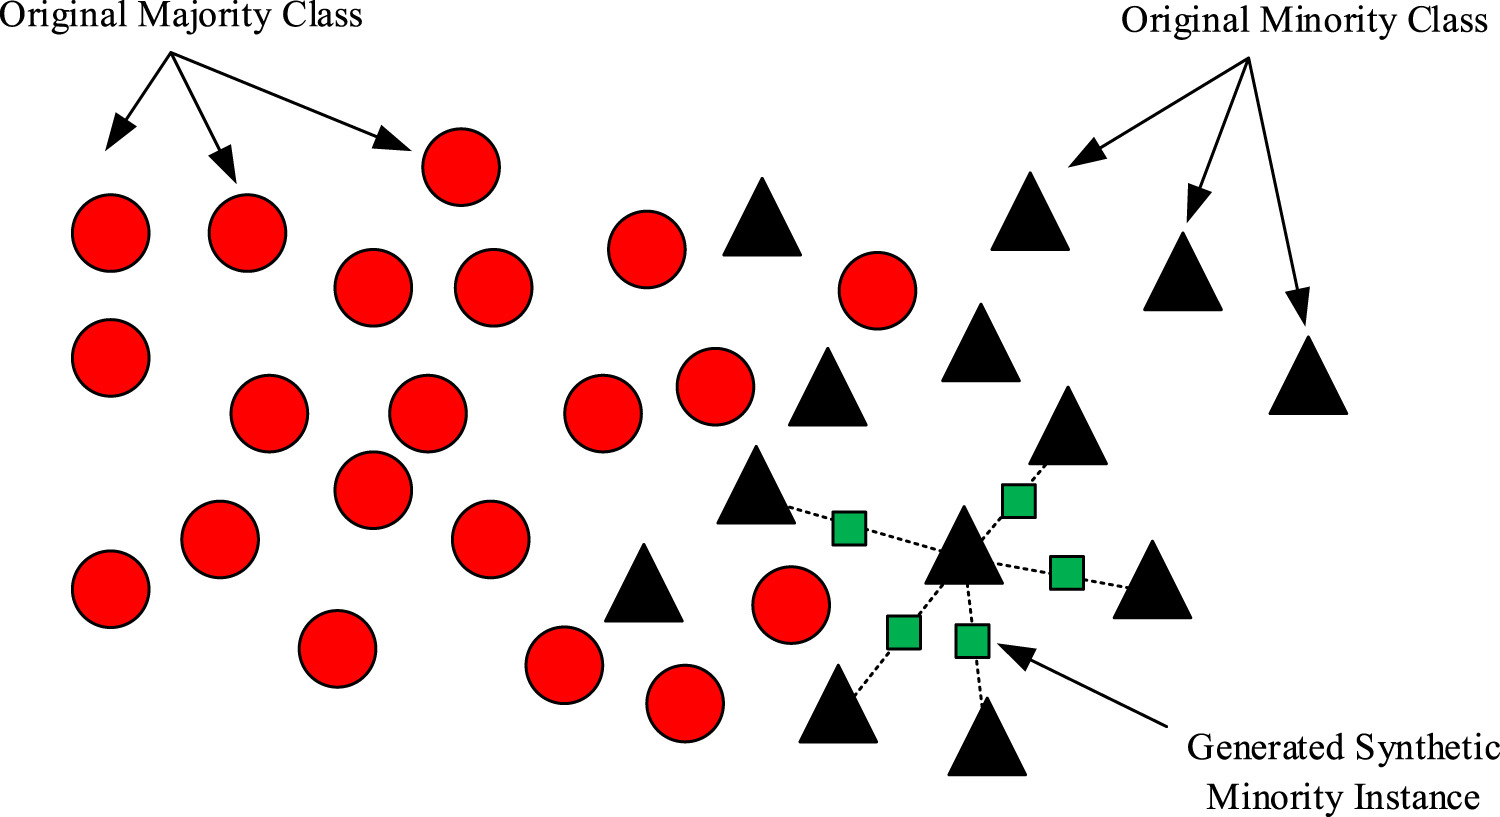
\includegraphics[width=0.7\textwidth]{images/smote.jpg}
\caption{Synthetic Minority Over-Sampling Technique}
\parencite{NNShen}
\label{fig:smote}
\end{figure}

\vspace{15pt}

\textcite{NNShen} compared their back propagation NN, with PSO weight determination, model against 7 other techniques. These techniques included LDA, logistic regression (Log R in Figure \ref{fig:shen}), SVM, a back propagation NN that did not use the PSO weight determination method (BP in Figure \ref{fig:shen}), KNN, classification trees (CT in Figure \ref{fig:shen}), and a Naive Bayes classifier (NB in Figure \ref{fig:shen}). Each model was trained on the same balanced dataset. Like \textcite{NNWest}, \textcite{NNShen} used 10-fold cross validation to test each developed model. Figure \ref{fig:shen} displays that their model out performed the other models in AUC, total accuracy, F1-score, and repaid accuracy (Type I Accuracy in the figure). The model did however not outperform all models in detecting defaulted credits (Type II Accuracy in the figure). 

\vspace{15pt}

\begin{figure}[!htb]
\centering
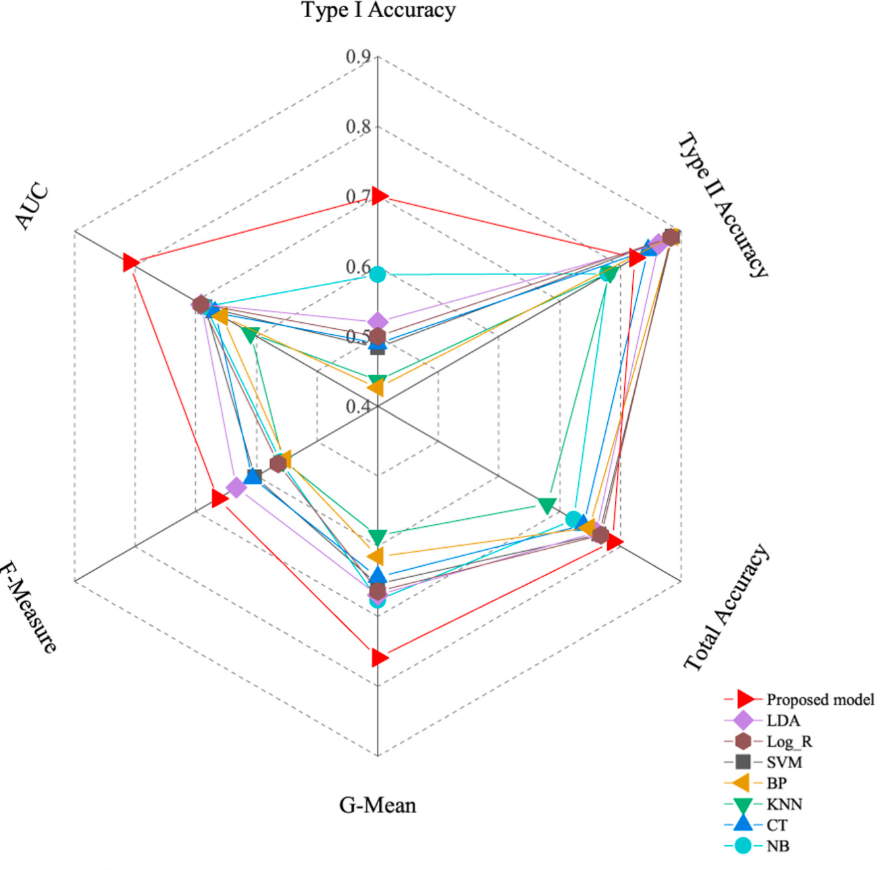
\includegraphics[width=0.7\textwidth]{images/shen.png}
\caption{The Results of the Research Conducted by \textcite{NNShen}}
\label{fig:shen}
\end{figure}

\vspace{15pt}

%---------------------------------------------------------------------------------------
%	SECTION 4
%---------------------------------------------------------------------------------------

\section{Ensemble Models}

There are two main methods used for ensemble modelling. The first is a parallel structure, which involves developing more than one model from training data and combining their outputs based on an ensemble strategy to produce a final prediction. The second method is a consequential structure, which involves feeding the output of one model into the next until a final outcome is produced. Figure \ref{fig:ensemble} visually displays the two main methods. 

\vspace{15pt}

\begin{figure}[!htb]
\centering
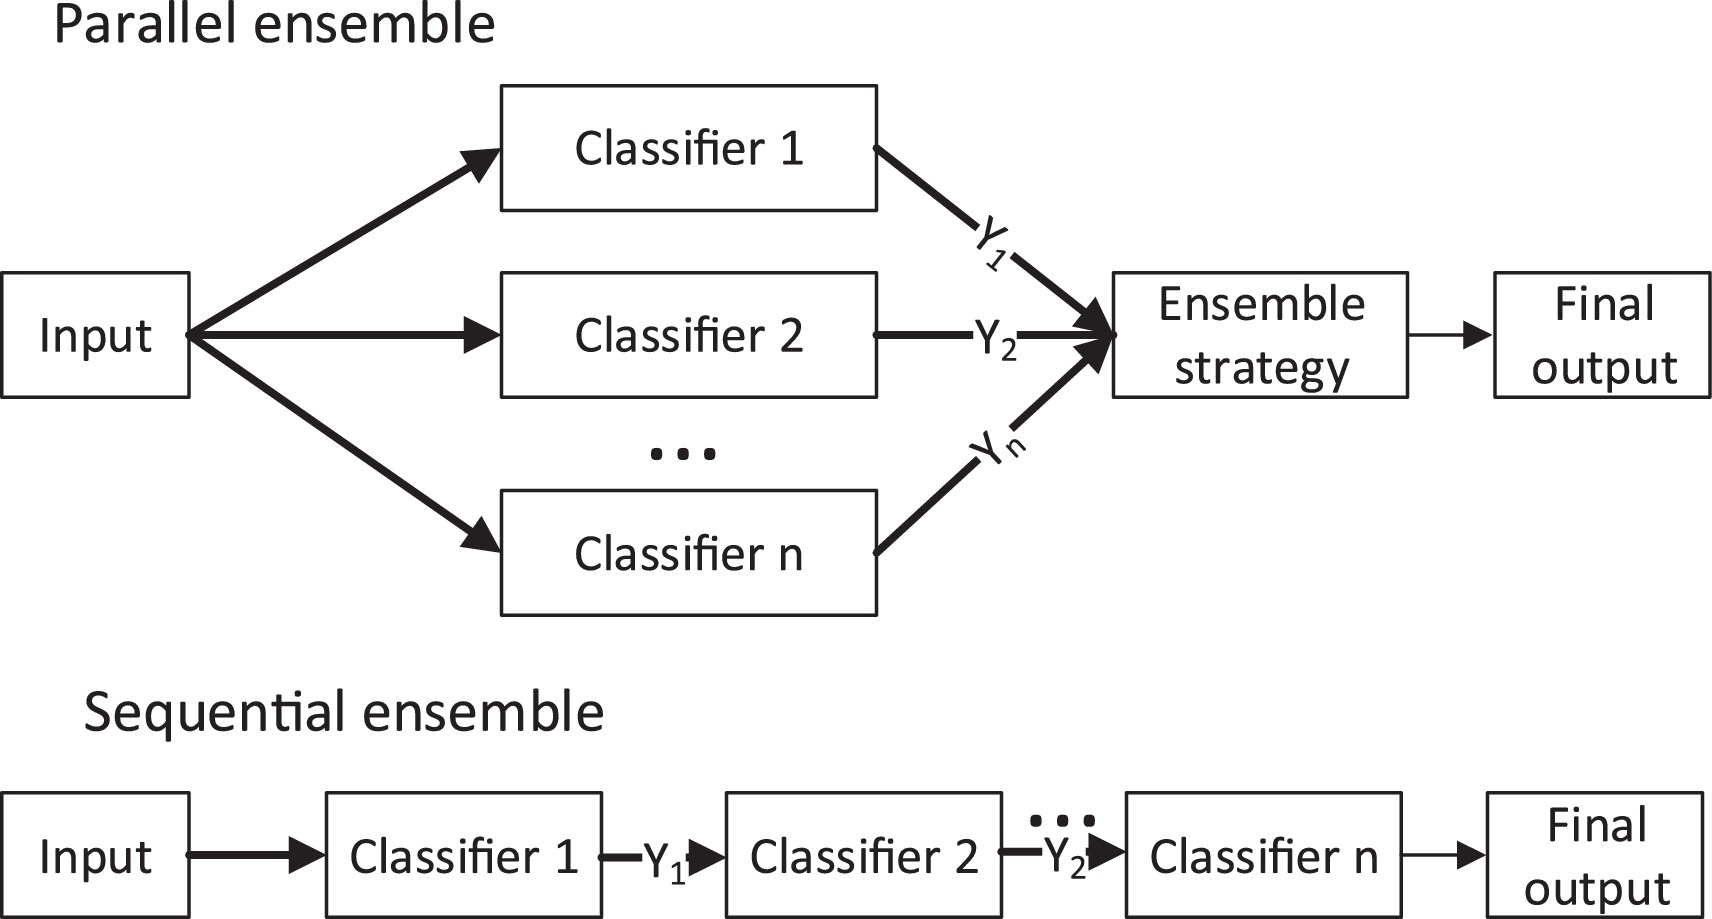
\includegraphics[width=0.6\textwidth]{images/ensemble.jpg}
\caption{Parallel and Consequential Ensemble Models}
\parencite{Ensemble}
\label{fig:ensemble}
\end{figure}

\vspace{15pt}

\subsection{Bagging}

Bootstrap aggregating is one of the earliest parallel ensemble machine learning methods. It was first developed by \textcite{BagBri}. The method involves developing numerous base models of the same underlying structure. Each model is trained on a separate sub-dataset that is randomly drawn—with replacement—from the entire dataset. The models are combined using majority vote. \\

\textcite{BagWang} developed a bagging credit scoring model that used decision trees as the underlying base models. In order to further improve the performance of their model and to avoid redundant features impacting the model, when each new decision tree was trained on a sub-dataset not all features available features were used. Features were randomly sampled. This feature sampling technique is referred to as random subspace sampling. \\

\textcite{BagWang} used the same German credit provider dataset used by \textcite{NNWest} and \textcite{NNShen} to train their model. \textcite{BagWang} further developed a decision tree model, a random forest model, and a bagging model that did not make use of random subspace sampling for comparative purposes. The results from their research can be seen in Table \ref{table:bagging}. 


\vspace{15pt}

\begin{table}[H]
\begin{center}
\begin{tabular}{|c|c|c|c|} 
\hline
\multicolumn{1}{|c}{Model}  &\multicolumn{1}{|c|}{Total Accuracy (\%)}  &\multicolumn{1}{|c|}{Bad Accuracy (\%)} & \multicolumn{1}{c|}{Good Accuracy (\%)}\\
\hline
DT  & 72.10 &  46.80 & 72.94 \\
\hline
Random Forest & 77.05 & 43.72 & 90.48 \\
\hline
Bagging & 78.36 & 41.44 & 94.02 \\
\hline
Bagging with RS & 78.52 &  44.66 & 92.81 \\
\hline
\end{tabular}
\end{center}
\caption{Results of Research Conducted by \textcite{BagWang}}
\label{table:bagging}
\end{table}

\vspace{15pt}

Table \ref{table:bagging} displays that the bagging model that used random subspace sampling (RS) outperformed the other models in overall classification accuracy. It is interesting to note that although the decision tree model had the lowest overall accuracy, it performed best in terms of classifying loans that were not repaid (true negatives). Table \ref{table:bagging} further displays that all models developed by \textcite{BagWang} had low specificity (classifying loans that were not repaid as bad loans) rates. 


\subsection{Boosting}

Boosting is a sequential ensemble machine learning technique that involves altering the weights of samples in training datasets based on the errors of previously created classifiers. Misclassified samples in the training set are assigned with higher weights. A weighted voting scheme is then applied to produce a final model \parencite{BoostingFreund}. \\

\textcite{Ensemble} used extreme gradient boosting (XGBoost) to develop a credit repayment classification model. New base models in the XGBoost algorithm predict the residuals of previous base models in the sequence and add the outputs of each model are then added together to produce a final prediction. The algorithm uses gradient descent to minimise a defined loss function \parencite{BoostingCowan}. \\

The base models used in \textcite{Ensemble} were decision trees. The hyper-parameters of their XGBoost model were adaptively tuned using Bayesian optimisation, which involved mapping each hyper-parameter to the loss function and iteratively finding the local hyper-parameter function which minimised the loss function of the XGBoost model. \\

They further developed baseline models and used other hyper-parameter tuning methods to assess the performance of the model they developed. The XGBoost model developed outperformed bagging, decision tree, logistic regression, neural network, random forest and support vector machine models in overall prediction accuracy, area under the curve, and Brier score. Furthermore, the XGBoost model developed using Bayesian hyper-parameter optimisation outperformed 4 XGBoost models in overall prediction accuracy, area under the curve, and Brier score that used a grid search, a manual search and a random search algorithm to tune their hyper-parameters respectively. All models developed by \textcite{Ensemble} were trained on five separate credit datasets. The metrics presented were an aggregation of each model's performance across all datasets. \\


%---------------------------------------------------------------------------------------
%	SECTION 5
%---------------------------------------------------------------------------------------

\section{Alternative Data in Credit Scoring}


In the decade between 1998 and 2008, the number of micro-finance institutions (MFIs) grew by 474\% and their number of customers increased by over 1000\%. MFIs generally provide a low amount, short term loans to lower income individuals. In less developed countries many first time customers for MFIs belong to the world's unbanked population. Furthermore, the credit bureaus in less developed countries do not necessarily store and release accurate and reliable data on the banked population. Traditional credit scoring models can therefore not always be applied to in these regions \parencite{MFICinca}.  \\


\textcite{MFIMLP} developed a multi-perceptron neural network that was trained on over 5,400 loans provided by Peruvian MFIs. The model used features that related to the personal characteristics of the loanees, the economic and financial ratios of the MFI the loan was provided by, the characteristics of the financial obligation (interest rate of loan, loan amount etc.), and variables related to the macroeconomic climate of Peru during the time time period of the loan. \\


\textcite{MFIMLP} developed a LDA model, logistic regression model, and multiple MLP models with varying architectures for comparative purposes. The architecture which lead to the most accurate MLP model was a 3 layer perceptron with 20 input nodes, 3 hidden nodes and a single output node. Each model was trained and its parameters tuned using 10-fold cross-validation. Table \ref{table:MFIMLP} displays the results of the LDA model, logistic regression and most accurate MLP models. 

\vspace{15pt}

\begin{table}[H]
\begin{center}
\begin{tabular}{|c|c|c|c|c|} 
\hline
\multicolumn{1}{|c}{Model}  &\multicolumn{1}{|c|}{AUC}  &\multicolumn{1}{|c|}{Bad Accuracy (\%)} & \multicolumn{1}{c|}{Good Accuracy (\%)} & \multicolumn{1}{c|}{Misclassification Costs}\\
\hline
LDA  & 0.9303 &  81.73 & 93.48 & 0.5143 \\
\hline
LR & 0.9322 & 79.04 & 94.06  & 0.5715 \\
\hline
MLP & 0.9543 & 84.70 & 92.24 & 0.4337 \\
\hline
\end{tabular}
\end{center}
\caption{Results of Research Conducted by \textcite{MFIMLP}}
\label{table:MFIMLP}
\end{table}

\vspace{15pt}

It can been seen in Table \ref{table:MFIMLP} that the MLP model has the highest AUC, the lowest misclassification cost and has the highest accuracy in terms of identifying loans that were not repaid as bad loans. \\

\textcite{BigDataMicroFiance} investigated the use of alternative
data sources to enhance the statistical and economic  performance of credit scoring models. They measured the impact of augmenting typical scoring features with features generated from cell phone data. The credit data was provided by a banking institution and the cell phone data was provided by a telecommunications provider. The data provided by the bank contained sociodemographic, account data and credit card repayment data for over 2 million customers. The data provided by the telecommunications company consisted of call data for over 90 million unique cell phone users. \\

Both data sources were used to generate a connected network between customers of both companies. Figure \ref{fig:network} displays an overall view of the network. Creditors were deemed to be a defaulter if they had missed 3 or more credit card repayments. 

\vspace{15pt}

\begin{figure}[!htb]
\centering
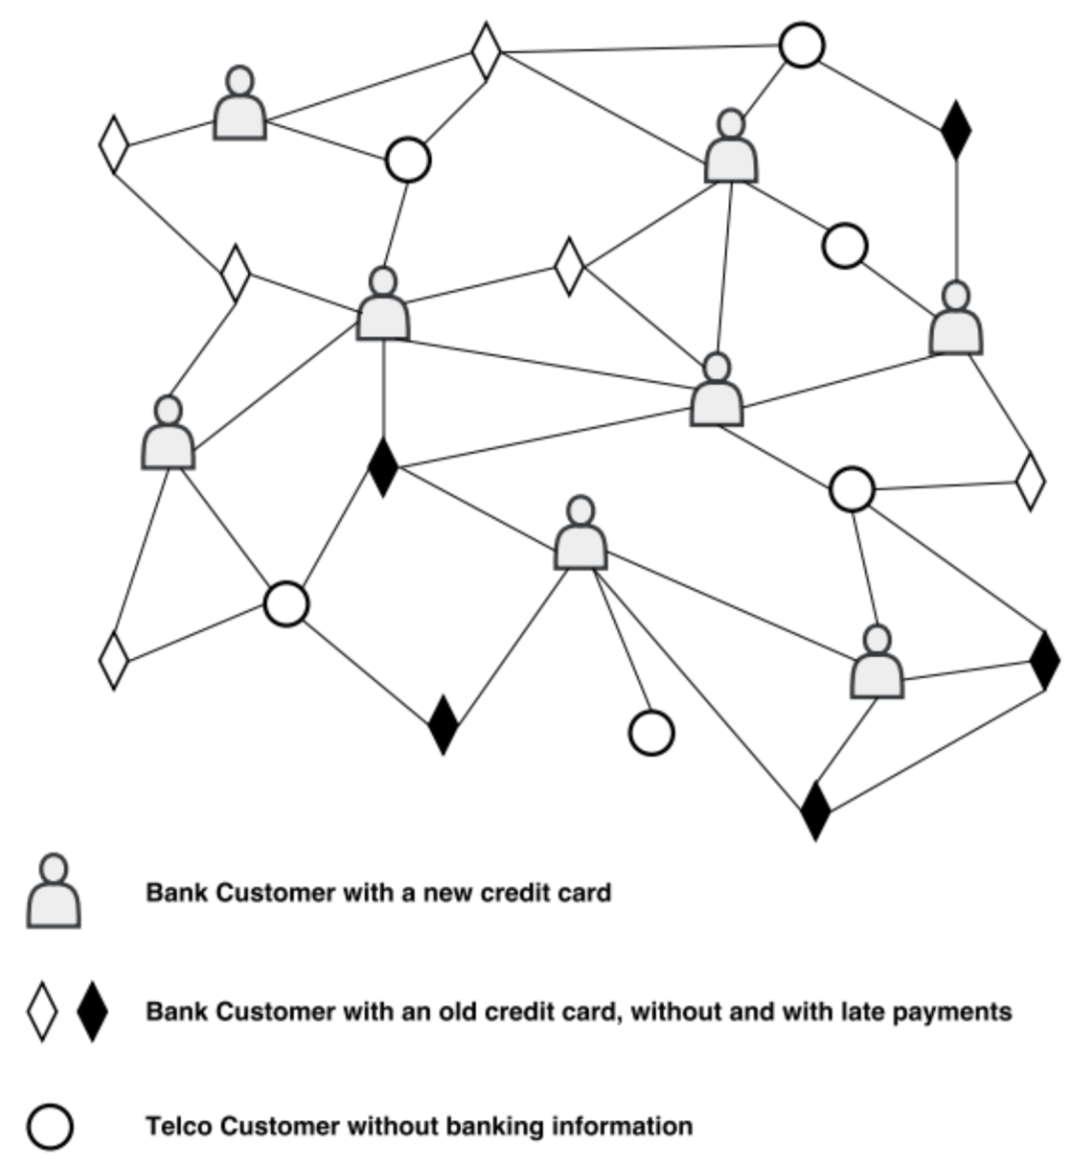
\includegraphics[width=0.6\textwidth]{images/network.png}
\caption{Network of Bank and Telecommunications Customers}
\parencite{BigDataMicroFiance}
\label{fig:network}
\end{figure}

\vspace{15pt}

 There were a total of 3 networks developed. One for each month that credit cards were disbursed to bank's customers. Bank customers and telecommunications customers that had shared a phone call within the three whole month period prior to the card acquisition month were connected. For each network \textcite{BigDataMicroFiance} used network analytics techniques to  propagate the influence of related defaulters throughout the network to produce influence scores. \\
 
 The call data features extracted from the network were as follows; the number and duration of incoming, outgoing and undirected phone calls taking place during the day and night and on different days of the week were computed. Furthermore, exposure scores to defaulted clients were calculated for each customer of each network using Personalised PageRank (PR) and Spreading Activation (SPA). \\
 
 
\textcite{BigDataMicroFiance} features listed above were combined with demographic and account data provided by the bank to build a credit scoring model for sample of bank's customers. This sample included only 22,000 of the banks 2 million customers. A logistic regression model, a decision tree model and a random forest model were developed for different feature samples. A sample was used that only contained sociodemographic (SD) features, another that only used credit based (CB) features, one that used both SD and CB features, one that used CB features and alternative features generated from the call data and network analysis, and finally one that used SD, CB, and alternative features generated from the call data and network analysis. The AUC of the different feature samples and models can be seen in Table \ref{table:alt}. 

\vspace{15pt}

\begin{table}[H]
\begin{center}
\begin{tabular}{|c|c|c|c|} 
\hline
\multicolumn{1}{|c}{Features}  &\multicolumn{1}{|c|}{Logistic regression}  &\multicolumn{1}{|c|}{Decision Trees} & \multicolumn{1}{c|}{Random Forest}\\
\hline
SD only  & 0.5869 &  0.7004 & 0.8993  \\
\hline
CB only & 0.5351 & 0.7043 & 0.8700  \\
\hline
SD and CB & 0.6115 & 0.7127 & 0.9227  \\
\hline
CB and Alternative & 0.5182 & 0.7307 & 0.0.9154  \\
\hline
SD,CB and Alternative & 0.6121 & 0.7263 & 0.9224  \\
\hline
\end{tabular}
\end{center}
\caption{Results of Research Conducted by \textcite{BigDataMicroFiance}}
\label{table:alt}
\end{table}

\vspace{15pt}
 
 
It can been seen in Table \ref{table:alt} that the performance of each
model type varies substantially. Furthermore, the logistic
regression models did not perform better when the
network-related features were used. This was believed to be due to linear regression models not being able to capture the non-linear behaviour of the network-related features. The best performing models were the random forest models. \\

The AUC test devised by \textcite{AUC} was used by \textcite{BigDataMicroFiance} to compare the performance of the random forest models. It was discovered that at a 95\% confidence level, the model produced both SD and CB features, the model produced using CB features and alternative features generated from the call data and network analysis, and the model produce using SD, CB, and alternative features showed a a significant statistical improvement in model performance compared to the models that used only SD and CB features.\\

However, there was no statistical difference between the model that used  SD and CB features, the model produced using CB features and alternative features generated from the call data and network analysis, and the model produce using SD, CB, and alternative features. 
